%Preamble
%Type (class) of document definition

\documentclass[12pt]{article}

%Packages used:

\usepackage[bottom]{footmisc} %footnote always at the bottom

\usepackage[utf8]{inputenc} %Always utf-8

\usepackage{hyperref} %Adds hyperlinks

\hypersetup{
    colorlinks=true,
    linkcolor=blue,
    filecolor=magenta,      
    urlcolor=cyan,
}

\usepackage{graphicx} %Adds images
\usepackage[english,brazilian]{babel}
\usepackage{xcolor} %Changes text color
\graphicspath{ {images/} } % Path to images folder
\usepackage{multicol} %Environments with multiple columns
\usepackage{mathptmx} %Several fonts (e.g. Times) and fontsizes
\usepackage{wrapfig} %Figures with text wrapping around them
\usepackage{xspace}
\usepackage{float} %allows for figures inside columns (no wrapping)
\usepackage{blindtext} %Generates dummy text
\usepackage{indentfirst} % indent first line of paragraph

\usepackage{listings} % lstlisting env: like verbatim env, but auto wraps lines
\lstset{
basicstyle=\small\ttfamily, %ttfamily is the typewriter font family used in LaTeX
columns=flexible,
breaklines=true,
backgroundcolor=\color{gray!10}
}


\usepackage{titlesec} % changes font sizes for sub/sub/sections

\titleformat{\section}
  {\normalfont\fontsize{15}{15}\bfseries}{\thesection}{1em}{}
\titleformat{\subsection}
  {\normalfont\fontsize{13}{15}\bfseries}{\thesubsection}{1em}{}
\titleformat{\subsubsection}
  {\normalfont\fontsize{12}{15}\bfseries}{\thesubsubsection}{1em}{}

\newcommand{\visible}[1]{\textbf{\textcolor{blue}{#1}}} %My first macro! It highlights some text.

\newcommand{\lightgray}{gray!20}

\newenvironment{myminipage}{
	\bigskip\begin{minipage}{\linewidth}
	}{
\end{minipage}\bigskip}

\newenvironment{boxed}
{\begin{tabular}{|p{\textwidth}|}
			\hline\\
		}
		{ 
			\\\\\hline
		\end{tabular}
}

\lstnewenvironment{rawlatex}{
	\lstset{
		basicstyle=\small\ttfamily,
		columns=flexible,
		breaklines=true,
		backgroundcolor=\color{gray!10}
	}
	}{}

\title{First document: \textit{Lorem Ipsum}\thanks{This template would not be completed without the \href{https://www.overleaf.com/}{Overleaf} \LaTeX{} editor and tutorials (from which a great part of this document has been ripped)} }
\author{Gabriel Alves Vieira (gavieira)\\
Contact: \href{mailto:gabrieldeusdeth@gmail.com}{gabrieldeusdeth@gmail.com} }
\date{\today}


%Document

\begin{document}

\maketitle
\thispagestyle{empty} %Removes first page number
    \begin{figure}[!h]
    	\centering
    	\begin{minipage}[c]{4cm} %c - aligns at center
    		\centering
    		
\includegraphics[scale=0.8]{overleaf}
    	\end{minipage}
    	\hspace{3cm}
    	\begin{minipage}[c]{4cm}
    		\centering
    		{\fontsize{60}{60}\selectfont{\LaTeX}}
    	\end{minipage}
    \end{figure}

\newpage

\tableofcontents
\listoffigures
\listoftables

\newpage

\begin{center}
    \title{{\fontsize{20}{60}\selectfont{\textbf{\textit{Lorem Ipsum}}}}}
\end{center}

\framebox{%
    \begin{minipage}{\linewidth}
    \textit{Lorem ipsum dolor sit amet, consectetur adipiscing elit, sed do eiusmod tempor incididunt ut labore et dolore magna aliqua. Ut enim ad minim veniam, quis nostrud exercitation ullamco laboris nisi ut aliquip ex ea commodo consequat. Duis aute irure dolor in reprehenderit in voluptate velit esse cillum dolore eu fugiat nulla pariatur. Excepteur sint occaecat cupidatat non proident, sunt in culpa qui officia deserunt mollit anim id est laborum.}\centering\end{minipage}}
    \\

\begin{multicols}{2}
\section{What is Lorem Ipsum?}
\textbf{Lorem Ipsum} is simply dummy text of the printing and typesetting industry. Lorem Ipsum has been the industry's standard dummy text ever since the 1500s, when an unknown printer took a galley of type and scrambled it to make a type specimen book. It has survived not only five centuries, but also the leap into electronic typesetting, remaining essentially unchanged. It was popularised in the 1960s with the release of Letraset sheets containing Lorem Ipsum passages, and more recently with desktop publishing software like Aldus PageMaker including versions of Lorem Ipsum.

\begin{figure}[H] % The H says that the image should NECESSARILY be placed HERE! (Needs float package to work in this multi-column env)
\centering

\includegraphics[width=0.5\linewidth]{ipsum_logo}
\caption[Shorter imagename]{\textit{Lorem ipsum} is part of pop culture\centering}
\end{figure}


%\begin{wrapfigure}{L}{0.4\textwidth}
%    
\includegraphics[width=0.4\textwidth]{ipsum_logo}
%    \caption{\textit{Lorem ipsum} is part of pop culture\centering}
%    \label{fig:lorem}
%\end{wrapfigure}

\section{Where does it come from?}
Contrary to popular belief, Lorem Ipsum is not simply random text. It has roots in a piece of classical Latin literature from 45 BC, making it over 2000 years old. Richard McClintock, a Latin professor at Hampden-Sydney College in Virginia, looked up one of the more obscure Latin words, consectetur, from a Lorem Ipsum passage, and going through the cites of the word in classical literature, discovered the undoubtable source. Lorem Ipsum comes from sections 1.10.32 and 1.10.33 of "de Finibus Bonorum et Malorum" (The Extremes of Good and Evil) by Cicero, written in 45 BC. This book is a treatise on the theory of ethics, very popular during the Renaissance. The first line of Lorem Ipsum, "Lorem ipsum dolor sit amet..", comes from a line in section 1.10.32.

The standard chunk of Lorem Ipsum used since the 1500s is reproduced below for those interested. Sections 1.10.32 and 1.10.33 from "de Finibus Bonorum et Malorum" by Cicero are also reproduced in their exact original form, accompanied by English versions from the 1914 translation by H. Rackham.

\section{%
Why do we use it?%
}

It is a long established fact that a reader will be distracted by the readable content of a page when looking at its layout. The point of using Lorem Ipsum is that it has a more-or-less normal distribution of letters, as opposed to using 'Content here, content here', making it look like readable English. Many desktop publishing packages and web page editors now use Lorem Ipsum as their default model text, and a search for 'lorem ipsum' will uncover many web sites still in their infancy. Various versions have evolved over the years (Figure \visible{\ref{fig:mussum}}), sometimes by accident, sometimes on purpose (injected humour and the like).

\end{multicols}

\begin{wrapfigure}{l}{0.5\textwidth}
    \begin{center}
    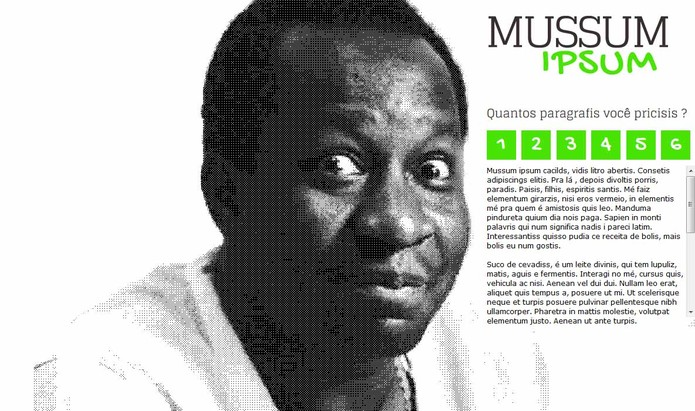
\includegraphics[width=0.5\textwidth]{mussum}
    \end{center}
    \caption{There are variants of \textit{Lorem ipsum}\centering}
    \label{fig:mussum}
\end{wrapfigure}\leavevmode

\section{Where can I get some?}
There are many variations of passages of Lorem Ipsum available, but the majority have suffered alteration in some form, by injected humour, or randomised words which don't look even slightly believable. If you are going to use a passage of Lorem Ipsum, you need to be sure there isn't anything embarrassing hidden in the middle of text. All the Lorem Ipsum generators on the Internet tend to repeat predefined chunks as necessary, making this the first true generator on the Internet. It uses a dictionary of over 200 Latin words, combined with a handful of model sentence structures, to generate Lorem Ipsum which looks reasonable. The generated Lorem Ipsum is therefore always free from repetition, injected humour, or non-characteristic words etc.

\newpage

\section{Basic  \LaTeX{}!}
\subsection{Images}
\subsubsection{Adding Images}

We will now look at how to add images to a LATEX document. On Overleaf, you will first have to \href{https://www.overleaf.com/learn/how-to/Including_images_on_Overleaf}{upload the images}.

\begin{myminipage}
Below is a example on how to include a picture: \\
\begin{rawlatex}
\documentclass{article}
\usepackage{graphicx}
\graphicspath{ {images/} }

	The universe is immense and it seems to be homogeneous, 
	in a large scale, everywhere we look at.
	
	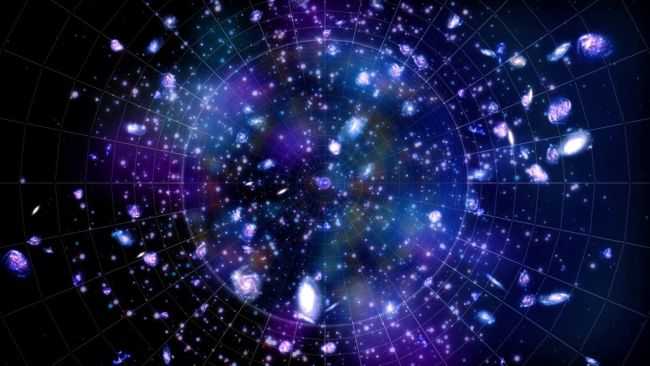
\includegraphics{universe}
	
	There's a picture of a galaxy above
	
\end{document}
\end{rawlatex}

Which outputs the following: \\

The universe is immense and it seems to be homogeneous, 
in a large scale, everywhere we look at.

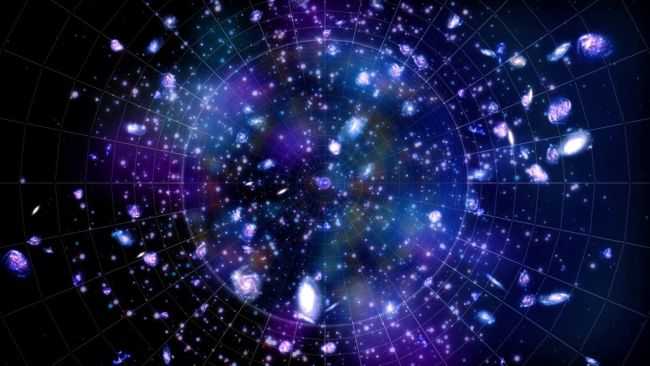
\includegraphics{universe}

There's a picture of a galaxy above \\

\end{myminipage}	

\LaTeX{} can not manage images by itself, so you will need to use a package. Packages can be used to change the default look of your \LaTeX{} document, or to allow more functionalities. In this case, you need to include an image in our document, so you should use the graphicx package. This package gives new commands, \lstinline!\includegraphics{...}! and \lstinline!\graphicspath{...}!. To use the graphicx package, include the following line in you preamble: \lstinline!\usepackage{graphicx}!

The command \verb+\graphicspath{ {images/} }+ tells LATEX that the images are kept in a folder named images under the current directory.
The \verb+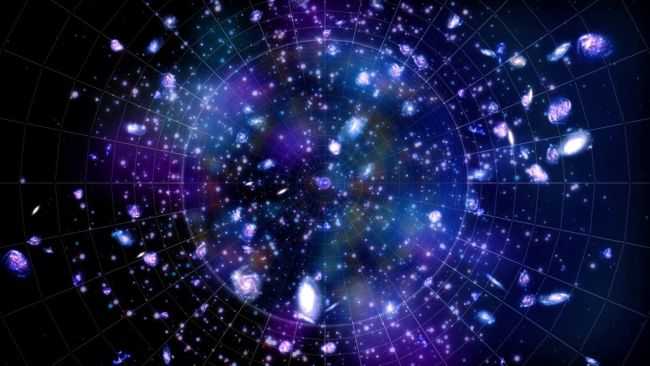
\includegraphics{universe}+ command is the one that actually included the image in the document. Here universe is the name of the file containing the image without the extension, then universe.PNG becomes universe. The file name of the image should not contain white spaces nor multiple dots\footnote{The file extension is allowed to be included, but it's a good idea to omit it. If the file extension is omitted it will prompt \LaTeX{} to search for all the supported formats. It is also usually recommended to use lowercase letters for the file extension when uploading image files. For more details see the section about \href{https://www.overleaf.com/learn/latex/Learn_LaTeX_in_30_minutes\#Generating_high-res_and_low-res_images}{generating high resolution and low resolution images}.}



\subsubsection{Captions, Labels and References}

Images can be captioned, labelled and referenced by means of the figure environment as shown below:\\

\begin{myminipage}
	Below is a example on how to include a picture: \\
	\begin{rawlatex}
		\begin{figure}[H]
			\centering
			\includegraphics[width=0.25\textwidth]{mesh}
			\caption{a nice plot}
			\label{fig:mesh1}
		\end{figure}
		
		As you can see in the figure \ref{fig:plot1}, the 
		function grows near 0. Also, in the page \pageref{fig:plot1} 
		is the same example.
	\end{rawlatex}
	
	\begin{figure}[H]
		\centering
		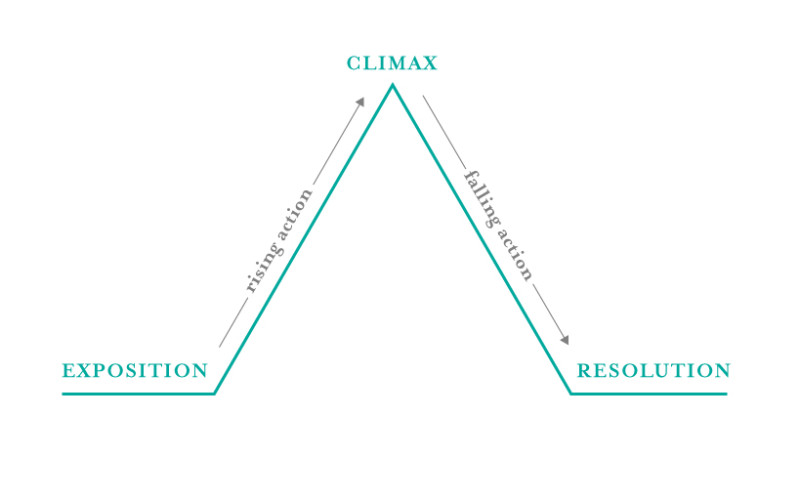
\includegraphics[width=0.25\textwidth]{plot}
		\caption{a nice plot}
		\label{fig:plot1}
	\end{figure}
	
	As you can see in the figure \ref{fig:plot1}, the 
	function grows near 0. Also, in the page \pageref{fig:plot1} 
	is the same example.
\end{myminipage}

There are three important commands in the example:
\begin{itemize}
	\setlength{\itemindent}{3em}
	\item \verb+\caption{a nice plot}+: As you may expect this command sets the caption for the figure. If you create a list of figures this caption will be used there. You can place it above or below the figure.
	\item \verb+\label{fig:mesh1}+: If you need to refer the image within your document, set a label with this command. The label will number the image, and combined with the next command will allow you to reference it.
	\item \verb+\ref{fig:mesh1}+: This code will be substituted by the number corresponding to the referenced figure.
\end{itemize}

When placing images in a LATEX document, we should always put them inside a figure environment or similar so that LATEX will position the image in a way that fits in with the rest of your text\footnote{If you are using captions and references on your own computer, you will have to compile the document twice for the references to work. Overleaf will do this for you automatically}.

\subsection{Lists}
    Lists are very simple to create in LaTeX. You can create lists using different list environments. Environments are sections of our document that you want to present in a different way to the rest of the document. They start with a \verb=\begin{...}= command and end with an \verb=\end{...}= command. 
    \subsubsection{Unordered Lists}
    Unordered lists are produced by the \textbf{itemize} environment: \bigskip
    
    \begin{minipage}[c]{\linewidth}
    \begin{lstlisting}
\begin{itemize}
\item The individual entries are indicated with a black dot a so-called bullet.
\item The text in the entries may be of any length.
\end{itemize}
    \end{lstlisting}
    \end{minipage}\bigskip
    
    \begin{minipage}{\linewidth}
    For instance:\\\\
    \fcolorbox{\lightgray}{\lightgray}{
    \begin{minipage}{\linewidth}
    \paragraph{Compras:}
    \begin{itemize}
        \item Arroz
        \item Feijão
        \item Temperos
        \begin{itemize}
            \item Açafrão
            \item Páprica
            \item Louro
            \item Sal do Himalaia
            \item Canela
        \end{itemize}
    \end{itemize}
    \end{minipage}}
    \end{minipage}


    \fcolorbox{\lightgray}{\lightgray}{
    \begin{minipage}{\linewidth}
    \paragraph{Sonhos:}
    \begin{itemize}
        \item Casa própria
        \item Emprego estável
            \begin{itemize}
                \item Bioinformata
                \item Developer
                \item Data scientist
            \end{itemize}
        \item PC gamer
    \end{itemize}
    \end{minipage}
    }
    
\subsubsection{Ordered Lists}
Ordered list have the same syntax inside a different environment. We make ordered lists using the enumerate environment:\bigskip

\begin{minipage}[c]{\linewidth}
    \begin{lstlisting}
\begin{enumerate}
  \item This is the first entry in our list
  \item The list numbers increase with each entry we add
\end{enumerate}
    \end{lstlisting}
    \end{minipage}\bigskip

    For instance:\bigskip
    
    \paragraph{Manhãs}
    \begin{enumerate}
        \item Levantar da cama
        \item Tomar banho
        \item Tomar café
        \item Escovar os dentes
        \item Sair para o trabalho
    \end{enumerate}

\subsection{Math}

One of the main advantages of \LaTeX is the ease at which mathematical expressions can be written. \LaTeX allows two writing modes for mathematical expressions: the \textbf{inline} mode and the \textbf{display} mode. The first one is used to write formulas that are part of a text. The second one is used to write expressions that are not part of a text or paragraph, and are therefore put on separate lines.\bigskip

\subsubsection{Inline Mode}

To put your equations in \textbf{inline} mode use one of these delimiters: \lstinline!\( ... \), $ ... $ or \begin{math} ... \end{math}!. They all work and the choice is a matter of taste.\bigskip

\textbf{Example:} To output Einstein's mass energy equivalence ($E=mc^2$) as inline text, you need to write it as \verb+$E=mc^2$+.\bigskip

\subsubsection{Displayed Mode}

The \textbf{displayed} mode has two versions: numbered and ununmbered. Take the following \LaTeX{} code\footnote{\textit{equation}* environment is provided by an external package, consult the \href{https://www.overleaf.com/learn/latex/Aligning\%20equations\%20with\%20amsmath}{amsmath article}. Since many math mode commands require this package, be sure to include it when writing math.}:\bigskip

\begin{minipage}{\linewidth}
\hrule

\begin{lstlisting}
The mass-energy equivalence is described by the famous equation

\[ E=mc^2 \]

discovered in 1905 by Albert Einstein. 
In natural units ($c = 1$), the formula expresses the identity

\begin{equation}
E=m
\end{equation}
\end{lstlisting}
\hrule
\end{minipage}
\bigskip


\begin{minipage}{\linewidth}

Which will generate the following text when interpreted by \LaTeX{}:\bigskip

\hrule\bigskip
The mass-energy equivalence is described by the famous equation

\[ E=mc^2 \]

discovered in 1905 by Albert Einstein. 
In natural units ($c = 1$), the formula expresses the identity

\begin{equation}
E=m
\end{equation}
\hrule
\end{minipage}\bigskip

The possibilities with math in \LaTeX{} are endless and it is impossible to list them all here. Check the \href{https://www.overleaf.com/learn/latex/Learn_LaTeX_in_30_minute}{Overleaf tutorial} for a list of other articles on \LaTeX{} math packages and formatting.

\subsection{Basic Formating}

\subsubsection{Abstracts}

In scientific documents it's a common practice to include a brief overview of the main subject of the paper. In LaTeX there's the abstract environment for this. The abstract environment will put the text in a special format at the top of your document. 

\begin{abstract}
    \noindent This is an abstract. Normally, it introduces the main topic of the study, its methods, results and conclusions in a very concise, not referenced way.\centering
\end{abstract}

When writing the contents of your document, if you need to start a new paragraph you must hit the "Enter" key twice (to insert a double blank line). Notice that LaTeX automatically indents paragraphs.

To start a new line without actually starting a new paragraph insert a break line point, this can be done by \verb+\\+ (a double backslash as in the example) or the \verb+\newline+ command.

Care should be taken that multiple \verb+\\+ or \verb+\newlines+ are not used to "simulate" paragraphs with larger spacing between them, as this can interfere with LaTeX's typesetting algorithms. The recommended method to do so is to keep using double blank lines to create new paragraphs without any \verb+\\+, and then add \verb+\usepackage{parskip}+ to the preamble. You can find more information in the \hyperref[subsec:Parag-nwl]{Paragraphs and new lines} subsection.

\subsection{Chapters and Sections}


\begin{minipage}{\linewidth}
Commands to organize a document vary depending on the document type, the simplest form of organization is the sectioning, available in all formats. Example of this can be seen in the code below:

\rule[-.3\baselineskip]{\linewidth}{.1mm}
\begin{lstlisting}

\chapter{First Chapter}

\section{Introduction}

This is the first section.

Lorem  ipsum  dolor  sit  amet,  consectetuer  adipiscing  
elit.   Etiam  lobortisfacilisis sem.  Nullam nec mi et 
neque pharetra sollicitudin.  Praesent imperdietmi nec ante. 
Donec ullamcorper, felis non sodales...

\section{Second Section}

Lorem ipsum dolor sit amet, consectetuer adipiscing elit.  
Etiam lobortis facilisissem.  Nullam nec mi et neque pharetra 
sollicitudin.  Praesent imperdiet mi necante...

\subsection{First Subsection}
Praesent imperdietmi nec ante. Donec ullamcorper, felis non sodales...

\section*{Unnumbered Section}
Lorem ipsum dolor sit amet, consectetuer adipiscing elit.  
Etiam lobortis facilisissem
\end{lstlisting}
\rule[1cm]{\linewidth}{.1mm}
\end{minipage}

The command \verb+\section{}+ marks the beginning of a new section, inside the braces is set the title. Section numbering is automatic and can be disabled by including a * in the section command as \verb+\section*{}+. We can also have \verb+\subsection{}+s, and indeed \verb+\subsubsection{}+s. 


\begin{minipage}{\linewidth}
The basic levels of depth are listed below:

\begin{enumerate}
    \item \verb+\part{part}+
    \item \verb+\chapter{chapter}+
    \item \verb+\section{section}+
    \item \verb+\subsection{subsection}+
    \item \verb+\subsubsection{subsubsection}+
    \item \verb+\paragraph{paragraph}+
    \item \verb+\subparagraph{subparagraph}+
\end{enumerate}\bigskip

Note that \verb+\part+ and \verb+\chapter+ are only available in report and book document classes.
\end{minipage}

\subsection{Creating Tables}



\subsubsection{Creating a simple table in \LaTeX{}}

\begin{minipage}{\linewidth}
Below you can see the simplest working example of a table:\bigskip
\hrule
\begin{lstlisting}
\begin{center}
\begin{tabular}{ c c c }
 cell1 & cell2 & cell3 \\ 
 cell4 & cell5 & cell6 \\  
 cell7 & cell8 & cell9
\end{tabular}
\end{center}
\end{lstlisting}
\hrule
\end{minipage}\bigskip

\begin{minipage}{\linewidth}
That will render the following:\bigskip
\begin{center}
\begin{tabular}{ c c c }
 cell1 & cell2 & cell3 \\ 
 cell4 & cell5 & cell6 \\  
 cell7 & cell8 & cell9
\end{tabular}
\end{center}
\end{minipage}\bigskip

\begin{minipage}{\linewidth}
The tabular environment is the default LaTeX method to create tables. You must specify a parameter to this environment, in this case {c c c}. This tells LaTeX that there will be three columns and that the text inside each one of them must be centred. You can also use r to align the text to the right and l for left alignment. The alignment symbol \& is used to specify the breaks in the table entries. There must always be one less alignment symbol in each line than the number of columns. To go to the next line of your table, we use the new line command \verb+\\+. We wrap the entire table inside the center environment so that it will appear in the center of the page. 
\end{minipage}

\subsubsection{Adding Borders}

The tabular environment is more flexible, you can put separator lines in between each column:\bigskip

\begin{minipage}{\linewidth}
\hrule
\begin{lstlisting}
\begin{center}
\begin{tabular}{ |c|c|c| } 
 \hline
 cell1 & cell2 & cell3 \\ 
 cell4 & cell5 & cell6 \\ 
 cell7 & cell8 & cell9 \\ 
 \hline
\end{tabular}
\end{center}
\end{lstlisting}
\hrule
\bigskip
\begin{center}
\begin{tabular}{ |c|c|c| } 
 \hline
 cell1 & cell2 & cell3 \\ 
 cell4 & cell5 & cell6 \\ 
 cell7 & cell8 & cell9 \\ 
 \hline
\end{tabular}
\end{center}
\end{minipage}\bigskip

You can add borders using the horizontal line command \verb+\hline+ and the vertical line parameter \texttt{|}.
    \begin{itemize}
        \item \texttt{|c|c|c|}: This declares that three columns, separated by a vertical line, are going to be used in the table. The | symbol specifies that these columns should be separated by a vertical line.
        \item \verb+\hline+: This will insert a horizontal line. We have included horizontal lines at the top and bottom of the table here. There is no restriction on the number of times you can use \verb+\hline+.
    \end{itemize}
\bigskip    
\begin{minipage}{\linewidth}
Below you can see a second example:\bigskip
\hrule
\begin{lstlisting}
\begin{center}
 \begin{tabular}{||c c c c||} 
 \hline
 Col1 & Col2 & Col2 & Col3 \\ [0.5ex] 
 \hline\hline
 1 & 6 & 87837 & 787 \\ 
 \hline
 2 & 7 & 78 & 5415 \\
 \hline
 3 & 545 & 778 & 7507 \\
 \hline
 4 & 545 & 18744 & 7560 \\
 \hline
 5 & 88 & 788 & 6344 \\ [1ex] 
 \hline
\end{tabular}
\end{center}
\end{lstlisting}\hrule\bigskip

\begin{center}
 \begin{tabular}{||c c c c||} 
 \hline
 Col1 & Col2 & Col2 & Col3 \\ [0.5ex] 
 \hline\hline
 1 & 6 & 87837 & 787 \\ 
 \hline
 2 & 7 & 78 & 5415 \\
 \hline
 3 & 545 & 778 & 7507 \\
 \hline
 4 & 545 & 18744 & 7560 \\
 \hline
 5 & 88 & 788 & 6344 \\ [1ex] 
 \hline
\end{tabular}
\end{center}

\end{minipage}\bigskip
 
Creating tables in LaTeX can be a bit tricky sometimes, so you may want to use the \href{https://www.tablesgenerator.com/}{TablesGenerator.com} online tool to export LaTeX code for tabulars. The File - Paste table data option lets you copy and paste data from spreadsheet applications.

\subsubsection{Captions, labels and references}

You can caption and reference tables in much the same way as images. The only difference is that instead of the figure environment, you use the \texttt{table} environment. 

\begin{minipage}{\linewidth}
For instance...\bigskip
\hrule
\begin{lstlisting}
Table \ref{table:data} is an example of referenced \LaTeX{} elements.

\begin{table}[h!]
\centering
\begin{tabular}{||c c c c||} 
 \hline
 Col1 & Col2 & Col2 & Col3 \\ [0.5ex] 
 \hline\hline
 1 & 6 & 87837 & 787 \\ 
 2 & 7 & 78 & 5415 \\
 3 & 545 & 778 & 7507 \\
 4 & 545 & 18744 & 7560 \\
 5 & 88 & 788 & 6344 \\ [1ex] 
 \hline
\end{tabular}
\caption{Table to test captions and labels}
\label{table:data}
\end{table}
\end{lstlisting}
\hrule
\end{minipage}\bigskip

Table \ref{table:data} is an example of referenced \LaTeX{} elements\footnote{If you are using captions and references on your own computer, you will have to compile the document twice for the references to work. Overleaf will do this for you automatically.}

\begin{table}[h!]
	\centering
	\begin{tabular}{||c c c c||} 
		\hline
		Col1 & Col2 & Col2 & Col3 \\ [0.5ex] 
		\hline\hline
		1 & 6 & 87837 & 787 \\ 
		2 & 7 & 78 & 5415 \\
		3 & 545 & 778 & 7507 \\
		4 & 545 & 18744 & 7560 \\
		5 & 88 & 788 & 6344 \\ [1ex] 
		\hline
	\end{tabular}
	\caption{Table to test captions and labels}
	\label{table:data}
\end{table}

\subsubsection{The next thing...}

\newpage

\subsection{Paragraphs and new lines - unfinished}
\label{subsec:Parag-nwl}
This subsection will eventually be written


\subsubsection{Citation - unfinished}
This subsection will eventually be written


\end{document}